\chapter{Anexo} \label{chp:anexo}

\section{Materiales Desarrollados}
El código, junto con los datos específicos utilizados para generar los resultados para este trabajo se encuentran en https://github.com/krlokbrera/TDA\_CarloCabrera

\section{Uso de Inteligencia Artificial Generativa}

Para la realización de este trabajo, se ha hecho uso de herramientas de IA Generativa, como sería \textit{ChatGPT} \cite{chatgpt_conversacion}, para consultas relativas a la realización de la memoria (estructura de figura en overleaf, generación de citas).
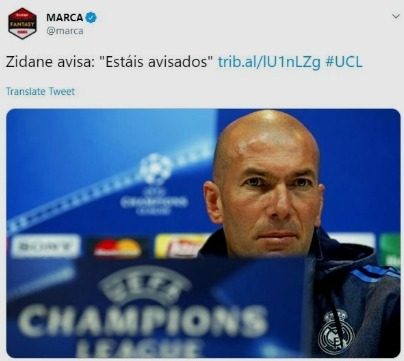
\includegraphics[scale=0.001]{images/anexo.jpg}

\section{Turnitin}

Tanto el informe de originalidad como el recibo digital se encuentran disponibles en el repositorio de Github https://github.com/krlokbrera/TDA\_CarloCabrera , más en concreto en la sección de documentos, junto con los archivos .tex utilizados para generar esta memoria.